% This file was converted to LaTeX by Writer2LaTeX ver. 1.6.1
% see http://writer2latex.sourceforge.net for more info
\documentclass[letterpaper]{article}
\usepackage[ascii]{inputenc}
\usepackage{amsmath}
\usepackage{amssymb,amsfonts,textcomp}
\usepackage[T1]{fontenc}
\usepackage[english]{babel}
\usepackage{color}
\usepackage{array}
\usepackage{hhline}
\usepackage{hyperref}
\hypersetup{pdftex, colorlinks=true, linkcolor=blue, citecolor=blue, filecolor=blue, urlcolor=blue, pdftitle=, pdfauthor=kenlo dinh-van, pdfsubject=, pdfkeywords=}
\usepackage[pdftex]{graphicx}
\providecommand\textsubscript[1]{\ensuremath{{}_{\text{#1}}}}
% Text styles
\newcommand\textstyleHeadingiiiChar[1]{\textrm{\textcolor[rgb]{0.12156863,0.21568628,0.3882353}{#1}}}
% Outline numbering
\setcounter{secnumdepth}{0}
% Page layout (geometry)
\setlength\voffset{-1in}
\setlength\hoffset{-1in}
\setlength\topmargin{2.54cm}
\setlength\oddsidemargin{2.54cm}
\setlength\textheight{22.86cm}
\setlength\textwidth{16.509998cm}
\setlength\footskip{0.0cm}
\setlength\headheight{0cm}
\setlength\headsep{0cm}
% Footnote rule
\setlength{\skip\footins}{0.119cm}
\renewcommand\footnoterule{\vspace*{-0.018cm}\setlength\leftskip{0pt}\setlength\rightskip{0pt plus 1fil}\noindent\textcolor{black}{\rule{0.25\columnwidth}{0.018cm}}\vspace*{0.101cm}}
% Pages styles
\makeatletter
\newcommand\ps@Standard{
  \renewcommand\@oddhead{}
  \renewcommand\@evenhead{}
  \renewcommand\@oddfoot{}
  \renewcommand\@evenfoot{}
  \renewcommand\thepage{\arabic{page}}
}
\makeatother
\pagestyle{Standard}
% List styles
\newcommand\liststyleWWNumii{%
\renewcommand\labelitemi{[F0B7?]}
\renewcommand\labelitemii{o}
\renewcommand\labelitemiii{[F0A7?]}
\renewcommand\labelitemiv{[F0B7?]}
}
\newcommand\liststyleWWNumi{%
\renewcommand\labelitemi{[F0B7?]}
\renewcommand\labelitemii{o}
\renewcommand\labelitemiii{[F0A7?]}
\renewcommand\labelitemiv{[F0B7?]}
}
\title{}
\author{kenlo dinh-van}
\date{2019-07-13}
\begin{document}
\clearpage\setcounter{page}{1}\pagestyle{Standard}
{\centering
\textbf{\textcolor{black}{SOEN 6011: Project Team C}}
\par}

{\centering
\textcolor{black}{Student N4: Kenlo DINH VAN (26641652)}
\par}


\bigskip

\section[1 Function Description]{\textbf{\textcolor{black}{1 Function Description}}}
\subsection[1.1 Logarithmic Function]{\textbf{\textcolor{black}{1.1 Logarithmic Function}}}
\begin{equation*}
\log _b(x)
\end{equation*}
\textcolor{black}{The }\textbf{\textcolor{black}{logarithmic}}\textcolor{black}{ function is the
}\textbf{\textcolor{black}{inverse}}\textcolor{black}{ of the exponential function, since it is a one-to-one function.
The graph of an inverse function is the reflection of the original function, using the line y = x as reflection axis.
John Napier expressed y as a function of x for the logarithm in 1614 resulting in:}

\begin{equation*}
\log _b(x)=y
\end{equation*}
\textcolor{black}{which can be read: ``x is equal to b (base) to the power y'', which is equivalent to {\textquotedbl}y
is the base-b logarithm of x.{\textquotedbl}}

{\centering  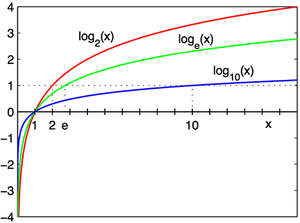
\includegraphics[width=5.44cm,height=4.038cm]{N4PB12-img001.png} \par}
\textstyleHeadingiiiChar{\textbf{\textcolor{black}{Domain}}\textcolor{black}{:}}\textcolor{black}{ x {\textgreater} 0
(set of positive real numbers) }

\textstyleHeadingiiiChar{\textbf{\textcolor{black}{Co-domain}}}\textcolor{black}{: Set of real numbers
}\textbf{\textcolor{black}{R}}

\textstyleHeadingiiiChar{\textbf{\textcolor{black}{Specificity of the base}}}\textcolor{black}{: b ${\neq}$ 1 and b
{\textgreater} 0}


\bigskip

\subsection[1.2 Unique characteristics]{\textbf{\textcolor{black}{1.2 Unique characteristics}}}
\textcolor{black}{Exponential expressions can be written as logarithmic expressions and logarithmic expressions can be
written as exponential expressions. ex: 3}\textcolor{black}{\textsuperscript{2}}\textcolor{black}{=9 ={\textgreater}
log}\textcolor{black}{\textsubscript{3}}\textcolor{black}{(9) = 2}

\liststyleWWNumii
\begin{itemize}
\item \textcolor{black}{when b = 10 the function is called common logarithm and denoted log(x)}
\item \textcolor{black}{when b = }\textit{\textcolor{black}{e}}\textcolor{black}{ = 2.7182818{\dots} the function is
called natural logarithm and denoted ln(x)}
\end{itemize}
\textstyleHeadingiiiChar{\textbf{\textcolor{black}{Logarithmic identities}}}\textcolor{black}{:}

\liststyleWWNumi
\begin{itemize}
\item \textcolor{black}{Product:\ \ \ \  } $\log _b(x\ast y)=\log _bx+\log _by$
\item \textcolor{black}{Quotient:\ \ \ \  } $\log _b(x/y)=\log _bx-\log _by$
\item \textcolor{black}{Power:\ \ \ \ \ \  } $\log _b(x^p)=p\log _bx$
\item \textcolor{black}{Root:\ \ \ \ \ \  } $\log _b\sqrt[p]x=\frac{\log _bx} p$
\end{itemize}
\section[2. Assumptions]{\textbf{\textcolor{black}{2. Assumptions}}}
\subsubsection[Assumption 1 ]{\textbf{\textcolor{black}{Assumption 1 }}}
\textcolor{black}{As of version 0, we assume that the user interface will be text based relying on console
input-output.}

\subsubsection[Assumption 2 ]{\textbf{\textcolor{black}{Assumption 2 }}}
\textcolor{black}{The `system' refers to the scientific calculator, Eternity: Functions}

\section[3. Functional requirements]{\textbf{\textcolor{black}{3. Functional requirements}}}
\subsubsection[F4.0.v1 Function Selection ]{\textbf{\textcolor{black}{F4.0.v1 Function Selection }}}
\textcolor{black}{When the system starts, the interface should display the function name and allow the user to select
the logarithmic function.}

\subsubsection[F4.1.v1 Logarithm Base Initialization ]{\textbf{\textcolor{black}{F4.1.v1 Logarithm Base Initialization
}}}
\textcolor{black}{When the user selects the logarithmic function, the system should ask the user which base
}\textit{\textcolor{black}{b}}\textcolor{black}{ he wishes to use and set the base value.}

\subsubsection[F4.2.v1 Logarithm Base Validation]{\textbf{\textcolor{black}{F4.2.v1 Logarithm Base Validation}}}
\textcolor{black}{After the user inputs the base value }\textit{\textcolor{black}{b}}\textcolor{black}{, the system
should validate that }\textit{\textcolor{black}{b}}\textcolor{black}{ is a real positive number not equal to 1.}

\subsubsection[F4.3.v1 Logarithm Variable Initialization]{\textbf{\textcolor{black}{F4.3.v1 Logarithm Variable
Initialization}}}
\textcolor{black}{If the base }\textit{\textcolor{black}{b}}\textcolor{black}{ is valid, the system should ask the user
to input the value for variable }\textit{\textcolor{black}{x }}\textcolor{black}{and set it.}

\subsubsection[F4.4.v1 Logarithm Variable Validation]{\textbf{\textcolor{black}{F4.4.v1 Logarithm Variable Validation}}}
\textcolor{black}{After the user inputs the variable }\textit{\textcolor{black}{x}}\textcolor{black}{ value, the system
should validate that the variable }\textit{\textcolor{black}{x}}\textcolor{black}{ is a real positive number.}

\subsubsection[F4.5.v1 Logarithm Calculation]{\textbf{\textcolor{black}{F4.5.v1 Logarithm Calculation}}}
\textcolor{black}{If the variable }\textit{\textcolor{black}{x}}\textcolor{black}{ is valid, the system should calculate
the logarithm of }\textit{\textcolor{black}{x}}\textcolor{black}{ in base
}\textit{\textcolor{black}{b,}}\textcolor{black}{ without relying on java built-in functions, and store the result.}

\subsubsection[F4.6.v1 Result Display]{\textbf{\textcolor{black}{F4.6.v1 Result Display}}}
\textcolor{black}{After the calculation completes, the system should display the result on the user interface.}

\section[4. References]{\textbf{\textcolor{black}{4. References}}}
\textcolor{black}{[1] }\url{https://en.wikipedia.org/wiki/Logarithm}

\textcolor{black}{[2] }\url{http://dwb4.unl.edu/Chem/CHEM869R/CHEM869RMats/Logs/Logs.html}


\bigskip


\bigskip


\bigskip
\end{document}
